\documentclass[10pt, mathserif]{beamer}	% font and size
\mode<presentation>
{
	\setbeamercovered{dynamic}	% translucent when using pause
	\setbeamertemplate{navigation symbols}{}	% hide navigation bars
	\setbeamertemplate{caption}[numbered]	% numerate captions
	\setbeamertemplate{background}{
\includegraphics[height=\paperheight]{ISEE.pdf}}	% set background image
	\setbeamertemplate{footline}{\footnotesize \insertframenumber/\inserttotalframenumber \hfill}	% display page number at bottom left corner	
}
\usepackage{CJKutf8}	% encode for Chinese
\usepackage{times}		% font for english
\usepackage{amsmath, amsfonts, amssymb}	% math equations, symbols
\usepackage[english]{babel}
\usepackage{color}		% color content
\usepackage{graphicx}	% import figures
\usepackage{url}		% hyperlinks
\usepackage{bm}			% bold type for equations
\usepackage{hyperref}	% bookmarks
\hypersetup{bookmarks, unicode}	% unicode

\newcommand{\ftitle}[1]{\frametitle{\hspace{4ex} {#1}}}	% userdefine frametitle

\begin{document}
\begin{CJK}{UTF8}{song}	% all Chinese should be enclosed between the commands

\title[abbreviation]{ Information Maximization Approach }
\author{ 薛盛可 \\ xueshengke@zju.edu.cn}
\institute[ISEE]{\normalsize College of Information Science and Electronic Engineering \\~\\Zhejiang University}
\date{Spring, 2016}

\begin{frame}
	\titlepage
\end{frame}

\begin{frame}
	\ftitle{Objective}
	In terms of training neural networks, the most common way we take is \emph{Gradient Descent Method}. It has been widely used in researches indeed. \\
	~\\
	%Hereby, I am about to introduce you 
	An original method {\color{red}Information Maximization Approach} \footnote{A.~J. Bell and T.~J. Sejnowski, ``An information-maximization approach to blind
		separation and blind deconvolution,'' {\em Neural computation}, vol.~7,
		no.~6, pp.~1129--1159, 1995.} that is hypothesized to training a neural network.
	%My presentation contains two parts. First, I will show you the inference of the approach with an example. Then, give you the steps about how the approach be added into the training procedure.
\end{frame}

\AtBeginSection[]
{
\begin{frame}
   	\ftitle{Outline}
    \tableofcontents[currentsection, currentsubsection]
\end{frame}
}

\section{Inference}
\begin{frame}
	\ftitle{Information Maximization}
	\begin{figure}[htbp]
		\centering
		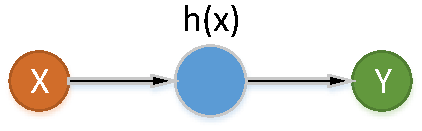
\includegraphics[width=0.4\textwidth]{mutual_information.pdf}
		\caption{Input X, output Y.}
	\end{figure}
	To maximize the mutual information between output Y and input X, which is defined as
	\begin{align}
	I({Y},{X}) &= H({Y})-H({Y} \mid {X}), \label{eq:I_Y_X} \\
	\frac{\partial}{\partial {w}} I({Y},{X}) &= \frac{\partial}{\partial {w}} H({Y}).
	\end{align}
	Maximize the mutual information is equivalent to maximize the entropy of output alone.
\end{frame}

\begin{frame}
	\ftitle{Example}
	We interpret the idea through an example as shown in Fig.~\ref{fig:network},
	\begin{itemize}
		\item $f_x(x)$ is the probability density function of input $x$.
		\item $f_y(y)$ is the probability density function of output $y$.
		\item $h(x)=1/(1+e^{-(ax+b)})$ is an adjustable activation function.
	\end{itemize}
	\begin{figure}[htbp]
		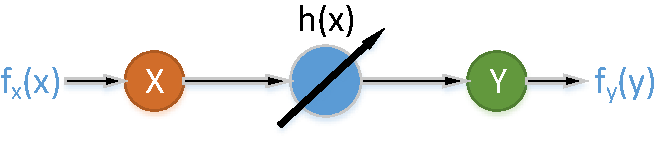
\includegraphics[width=0.6\textwidth]{network.pdf}
		\caption{One input and one output.} \label{fig:network}
	\end{figure}
\end{frame}

\begin{frame}
	\ftitle{Derivation}
	After a certain process of deduce,
	\begin{align}
		f_y(y) &= \frac{f_x(x)}{|\partial y/\partial x|},\ H(y)=E[\ln |\partial y/\partial x|] - E[\ln f_x(x)],\\
		\Delta w & \varpropto \frac{\partial H}{\partial w} = \frac{\partial }{\partial w} \left( \ln \left| \frac{\partial y}{\partial x} \right| \right) = \left( \frac{\partial y}{\partial x} \right)^{-1} \frac{\partial }{\partial w} \left( \frac{\partial y}{\partial x} \right).
	\end{align}
	We conclude the {\color{red}learning rules} of information maximization approach,
	\begin{align}
		\Delta a \varpropto \frac{\partial H}{\partial a} &= \frac{1}{a} + x(1-2y).\\
		\Delta b \varpropto \frac{\partial H}{\partial b} &= 1-2y.
	\end{align}
	The effect of two rules will be demonstrated intuitively.
\end{frame}

\section{Illustration}
\begin{frame}
	\ftitle{Information Maximization}
	\begin{minipage}{\textwidth}
	\begin{figure}
		\centering
		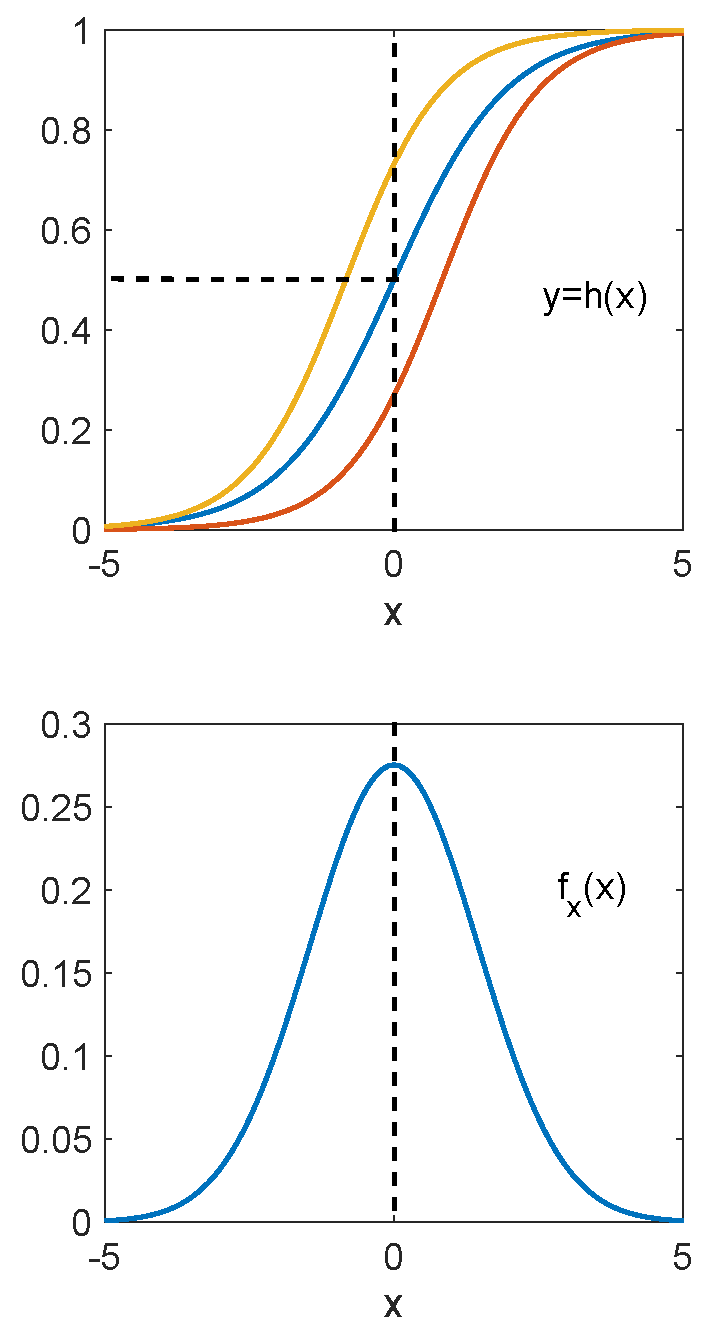
\includegraphics[width=0.3\textwidth]{example1.pdf}
		%\caption{}
		\label{fig:example}
	\end{figure}	
	\end{minipage}
	$\bullet$ \ $\Delta a$ rule scales the slope of sigmoid curve, to match the variance of \ $f_x(x)$. \\
	$\bullet$ \ $\Delta b$ rule shifts the sigmoid curve horizontally, to align the steepest part of sigmoid curve to the peak of \ $f_x(x)$. \\	
\end{frame}

\begin{frame}
	\ftitle{Conclusion}
	\begin{minipage}{\textwidth}
		\begin{figure}
			\centering
			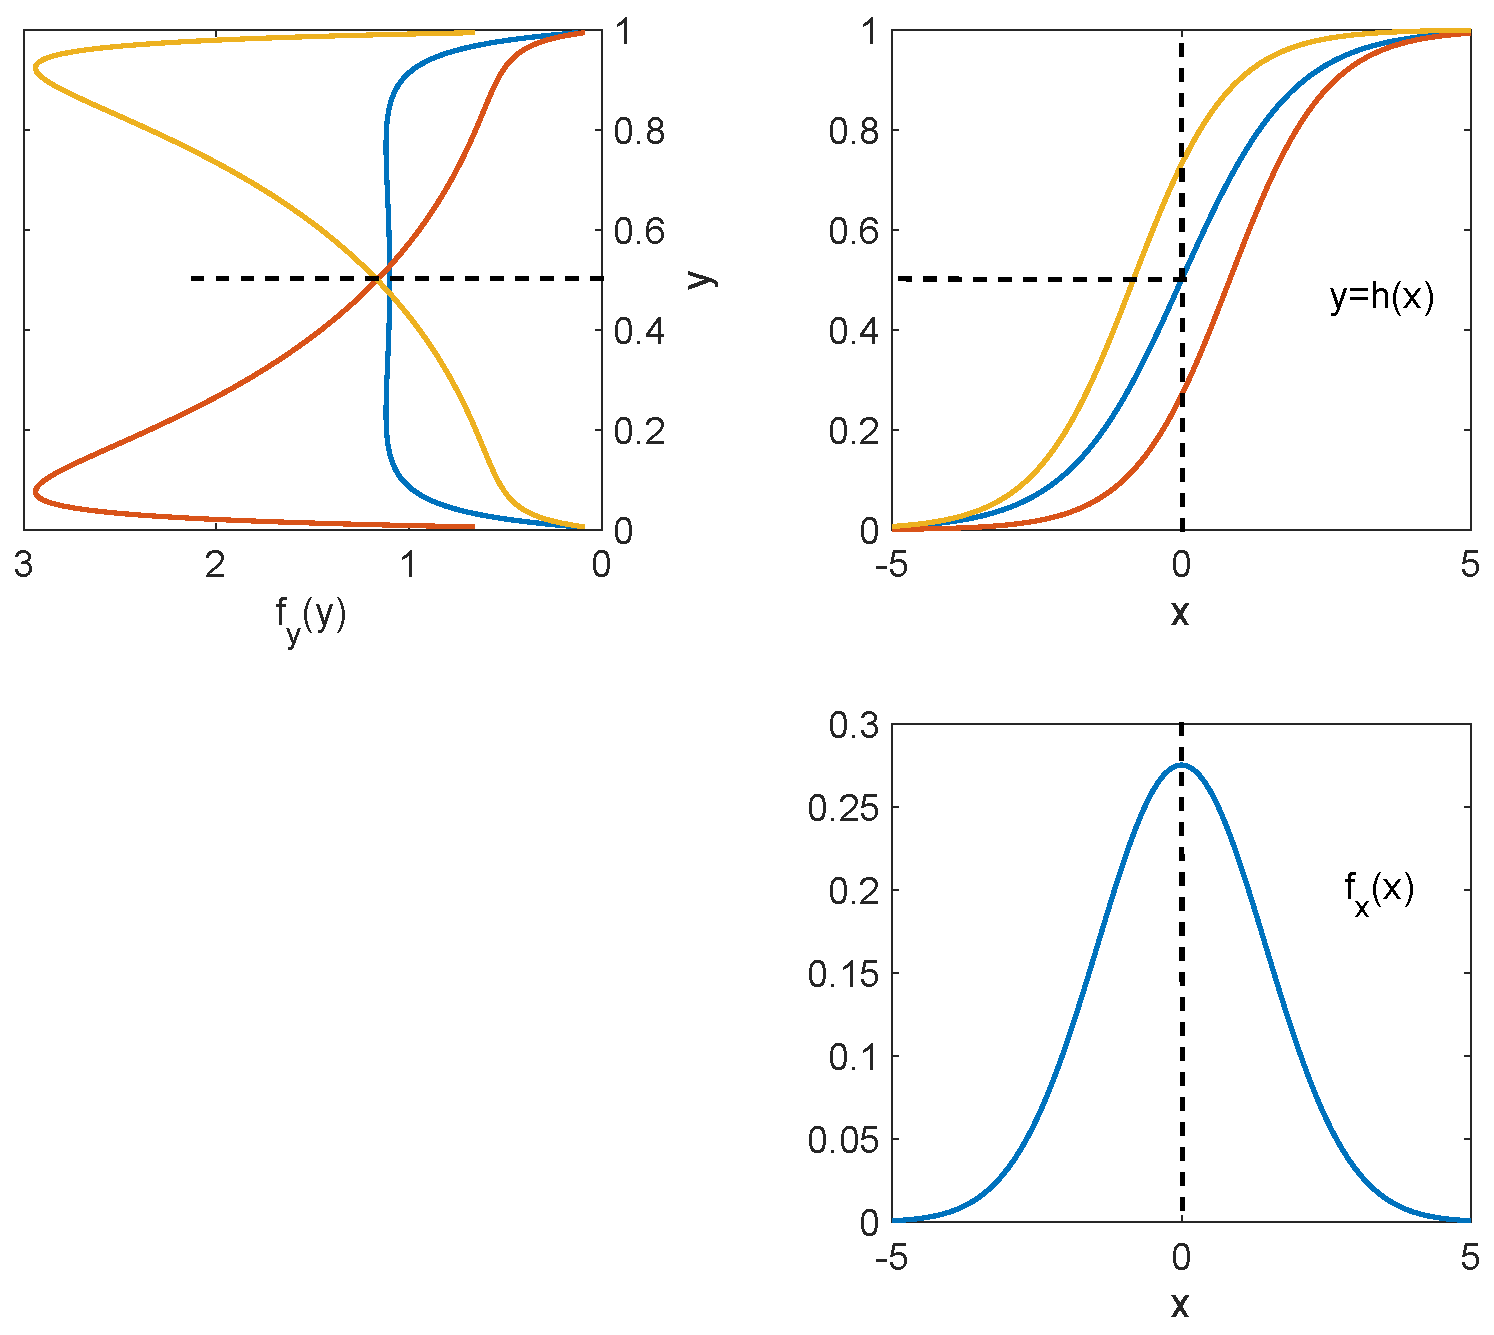
\includegraphics[width=0.65\textwidth]{example2.pdf}
			%\caption{}
			%\label{fig:example}
		\end{figure}	
	\end{minipage}
	Eventually, the effect {\color{red}produces an output ~$f_y(y)$~ }that is {\color{red}close to a flat unit distribution}, i.e., the {\color{red}maximum entropy distribution} without assuming any prior knowledge of the input distribution ~$f_x(x)$.
\end{frame}

\begin{frame}
	\ftitle{Training Algorithm}
	\begin{figure}[htbp]
		\centering
		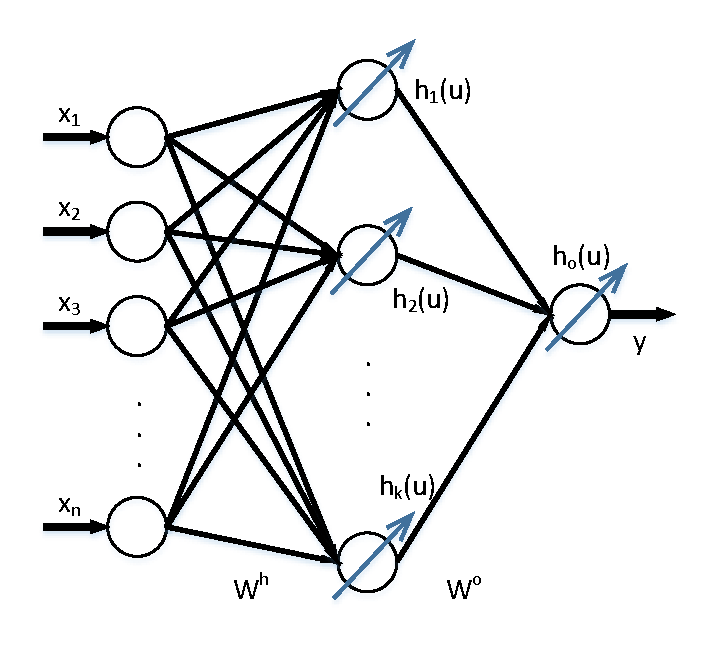
\includegraphics[width=0.5\textwidth]{fnn.pdf}
	\end{figure}
	New method to train a neural network that is composed of adjustable neurons: \\
	combine gradient descent method with {\color{red}information maximization approach}.
\end{frame}

%\section{References}
%\begin{frame}[allowframebreaks]
%	\ftitle{Bibliography}
%	中文内容显示
%    \label{Reference}
%    \bibliographystyle{apalike}
%    \bibliography{mybibliography}
%\end{frame}

\section*{Acknowledgement}
\begin{frame}
	\ftitle{End}
	\Huge Thanks for your listening. \\
	% Thank you very much!
\end{frame}

\end{CJK}
\end{document}
